\subsection*{Evaluation Plan Details}
In \autoref{sec:opt-and-tradeoffs} we highlight three plans (PLAN 1, 2, and 3), which provide useful performance trade-offs relative to baseline plans. The implementation details for each of these plans are described below.

\textbf{PLAN 1:} uses Mixtral-8x7B to convert each \texttt{TextFile} to the \texttt{Email} schema. It then uses Mixtral-8x7B again to apply the filter which checks whether or not the email refers to a fraudulent investment scheme. Finally, this plan uses gpt-3.5-turbo to determine whether or not the email is referring to a news article or is written by someone outside of Enron. A depiction of the plan is shown below:

\lstset{style=mystyle}
\begin{lstlisting}
 0. MarshalAndScanDataOp -> File 

 1. File -> InduceFromCandidateOp -> TextFile 
    Using hardcoded function
    (contents,filena...) -> (contents,filena...)

 2. TextFile -> InduceFromCandidateOp -> Email 
    Using Model.MIXTRAL
    Token budget: 1.0
    Query strategy: QueryStrategy.BONDED_WITH_FALLBACK
    (contents,filena...) -> (contents,filena...)

 3. Email -> FilterCandidateOp -> Email 
    Using Model.MIXTRAL
    Filter: "The email refers to a fraudulent scheme (i.e., "Raptor", ...)"
    (contents,filena...) -> (contents,filena...)

 4. Email -> FilterCandidateOp -> Email 
    Using Model.GPT_3_5
    Filter: "The email is not quoting from a news article..."
    (contents,filena...) -> (contents,filena...)
\end{lstlisting}

\textbf{PLAN 2:} uses gpt-3.5-turbo (with a token budget allowing it to process up to 50\% of the listing text) to convert each \texttt{RealEstateListingFiles} to the \texttt{TextRealEstateListing} schema. It then applies the UDF filters which check whether or not the listing is within two miles of MIT and in the user's price range. The plan then uses the gpt-4-vision-preview model to convert the schema to an \texttt{ImageRealEstateListing} (extracting the ``modern and attractive" and ``natural sunglight" attributes), before finally applying gpt-3.5-turbo to filter based on these attributes. A depiction of the plan is shown below:

\begin{lstlisting}
 0. MarshalAndScanDataOp -> RealEstateListingFiles 

 1. RealEstateListingFiles -> InduceFromCandidateOp -> TextRealEstateListing 
    Using Model.GPT_3_5
    Token budget: 0.5
    Query strategy: QueryStrategy.BONDED_WITH_FALLBACK
    (image_contents,...) -> (address,image_c...)

 2. TextRealEstateListing -> FilterCandidateOp -> TextRealEstateListing 
    Using None
    Filter: "<function get_logical_tree.<locals>.within_two_miles_of_mit"
    (address,image_c...) -> (address,image_c...)

 3. TextRealEstateListing -> FilterCandidateOp -> TextRealEstateListing 
    Using None
    Filter: "<function get_logical_tree.<locals>.in_price_range"
    (address,image_c...) -> (address,image_c...)

 4. TextRealEstateListing -> InduceFromCandidateOp -> ImageRealEstateListing 
    Using Model.GPT_4V
    Token budget: 1.0
    Query strategy: QueryStrategy.BONDED_WITH_FALLBACK
    (address,image_c...) -> (has_natural_sun...)

 5. ImageRealEstateListing -> FilterCandidateOp -> ImageRealEstateListing 
    Using Model.GPT_3_5
    Filter: "The interior is modern and attractive, and has lots of natural sunlight"
    (has_natural_sun...) -> (has_natural_sun...)
\end{lstlisting}

\textbf{PLAN 3:} uses Mixtral-8x7B to filter for the subset of tables which contain patient age information. It then uses Mixtral-8x7B once again (with a token budget allowing it to process up to 90\% of the input table data) to convert each input \texttt{Table} to the desired output \texttt{CaseData} schema. A depiction of the plan is shown below:

\begin{lstlisting}
 0. MarshalAndScanDataOp -> File 

 1. File -> InduceFromCandidateOp -> XLSFile 
    Using hardcoded function
    (contents,filena...) -> (contents,filena...)

 2. XLSFile -> InduceFromCandidateOp -> Table 
    Using hardcoded function
    (contents,filena...) -> (filename,header...)

 3. Table -> FilterCandidateOp -> Table 
    Using Model.MIXTRAL
    Filter: "The rows of the table contain the patient age"
    (filename,header...) -> (filename,header...)

 4. Table -> InduceFromCandidateOp -> CaseData 
    Using Model.MIXTRAL
    Token budget: 0.9
    Query strategy: QueryStrategy.BONDED_WITH_FALLBACK
    (filename,header...) -> (age_at_diagnosi...)
\end{lstlisting}

\begin{figure*}[h!]
    \begin{subfigure}[t]{0.48\textwidth}
        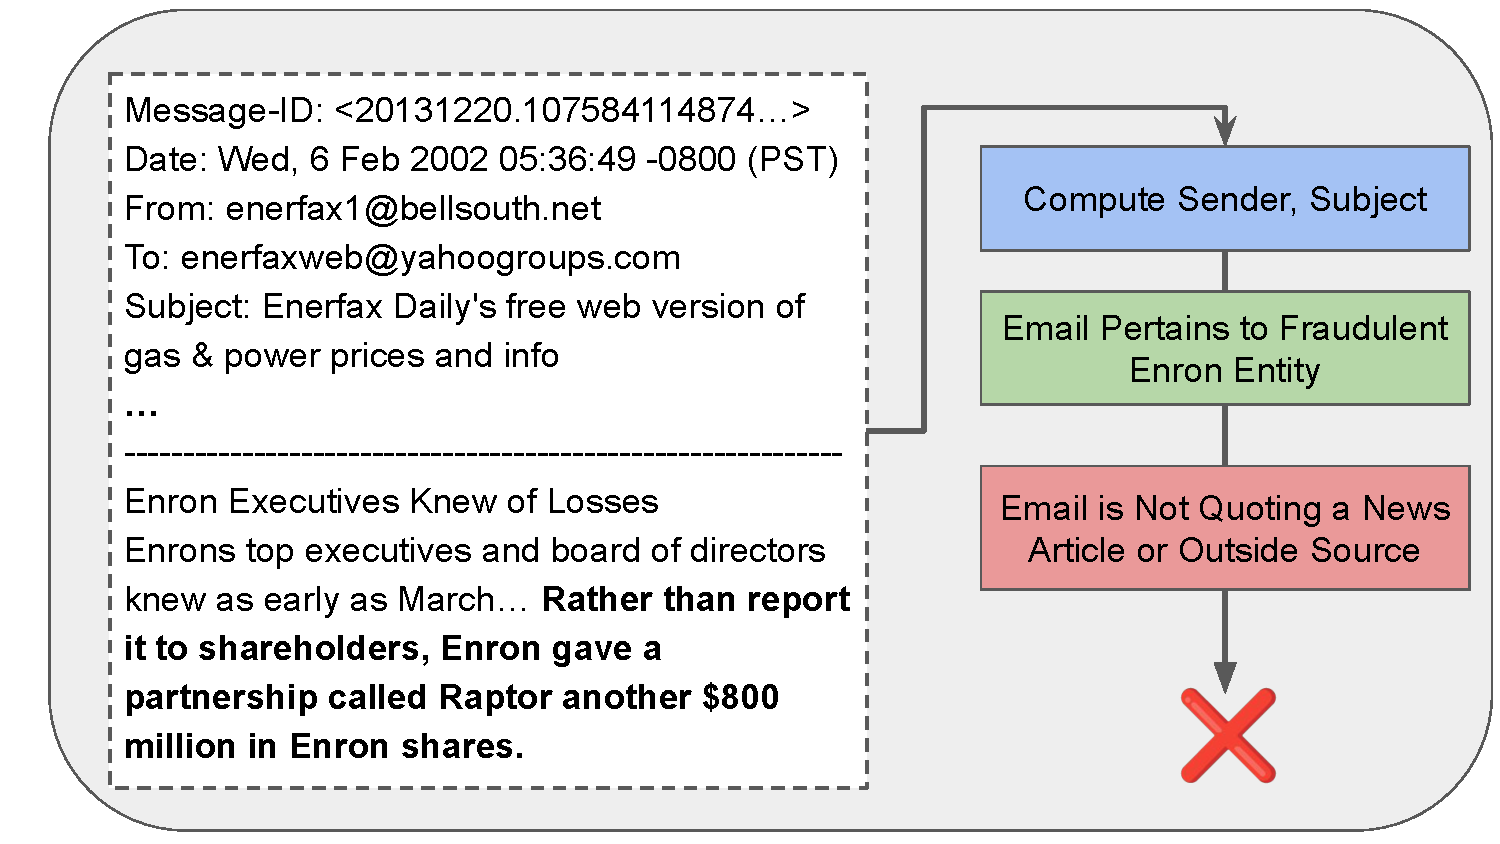
\includegraphics[width=\textwidth]{imgs/PZ-DIAGRAMS-enron-bad.pdf}
        \caption{Example of a negative entry in the Legal Discovery workload. This email does not meet the criteria set by the user's search because the email is quoting from a news article.}
    \label{fig:enron-incorrect}
    \end{subfigure}
    \hfill
    \begin{subfigure}[t]{0.48\textwidth}
        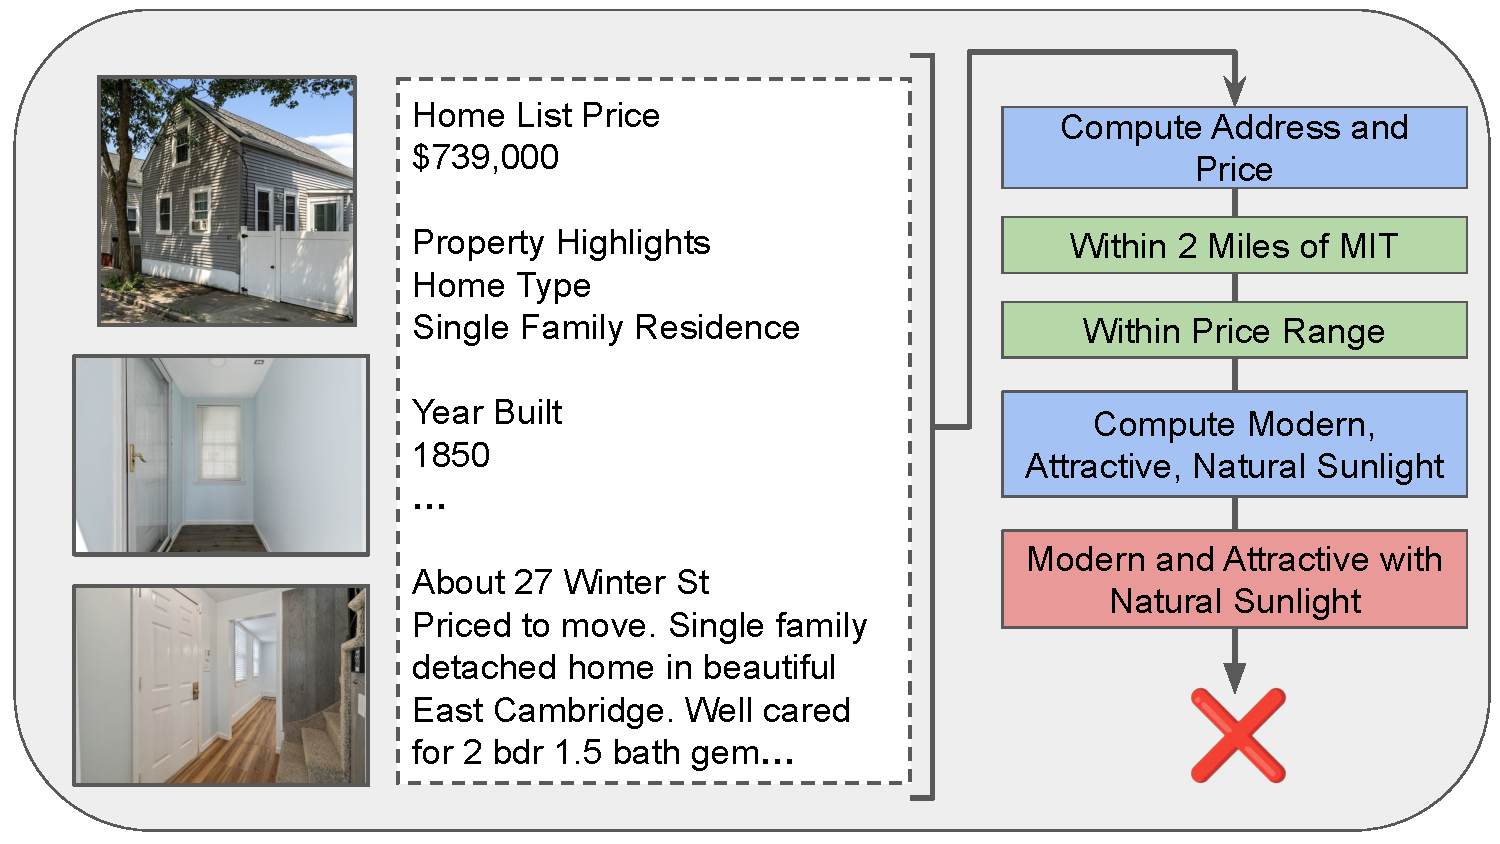
\includegraphics[width=\textwidth]{imgs/PZ-DIAGRAMS-real-estate-bad.pdf}
        \caption{Example of a negative entry in the Real Estate Search workload. This house does not meet the criteria set by the user’s search because the house is not considered to be modern and attractive.}
    \label{fig:real-estate-search-incorrect}
    \end{subfigure}
    \caption{Negative examples in the Legal Discovery and Real Estate Search workloads.}
    \label{fig:negative-examples}
\end{figure*}

% \begin{figure*}
%     \centering
%     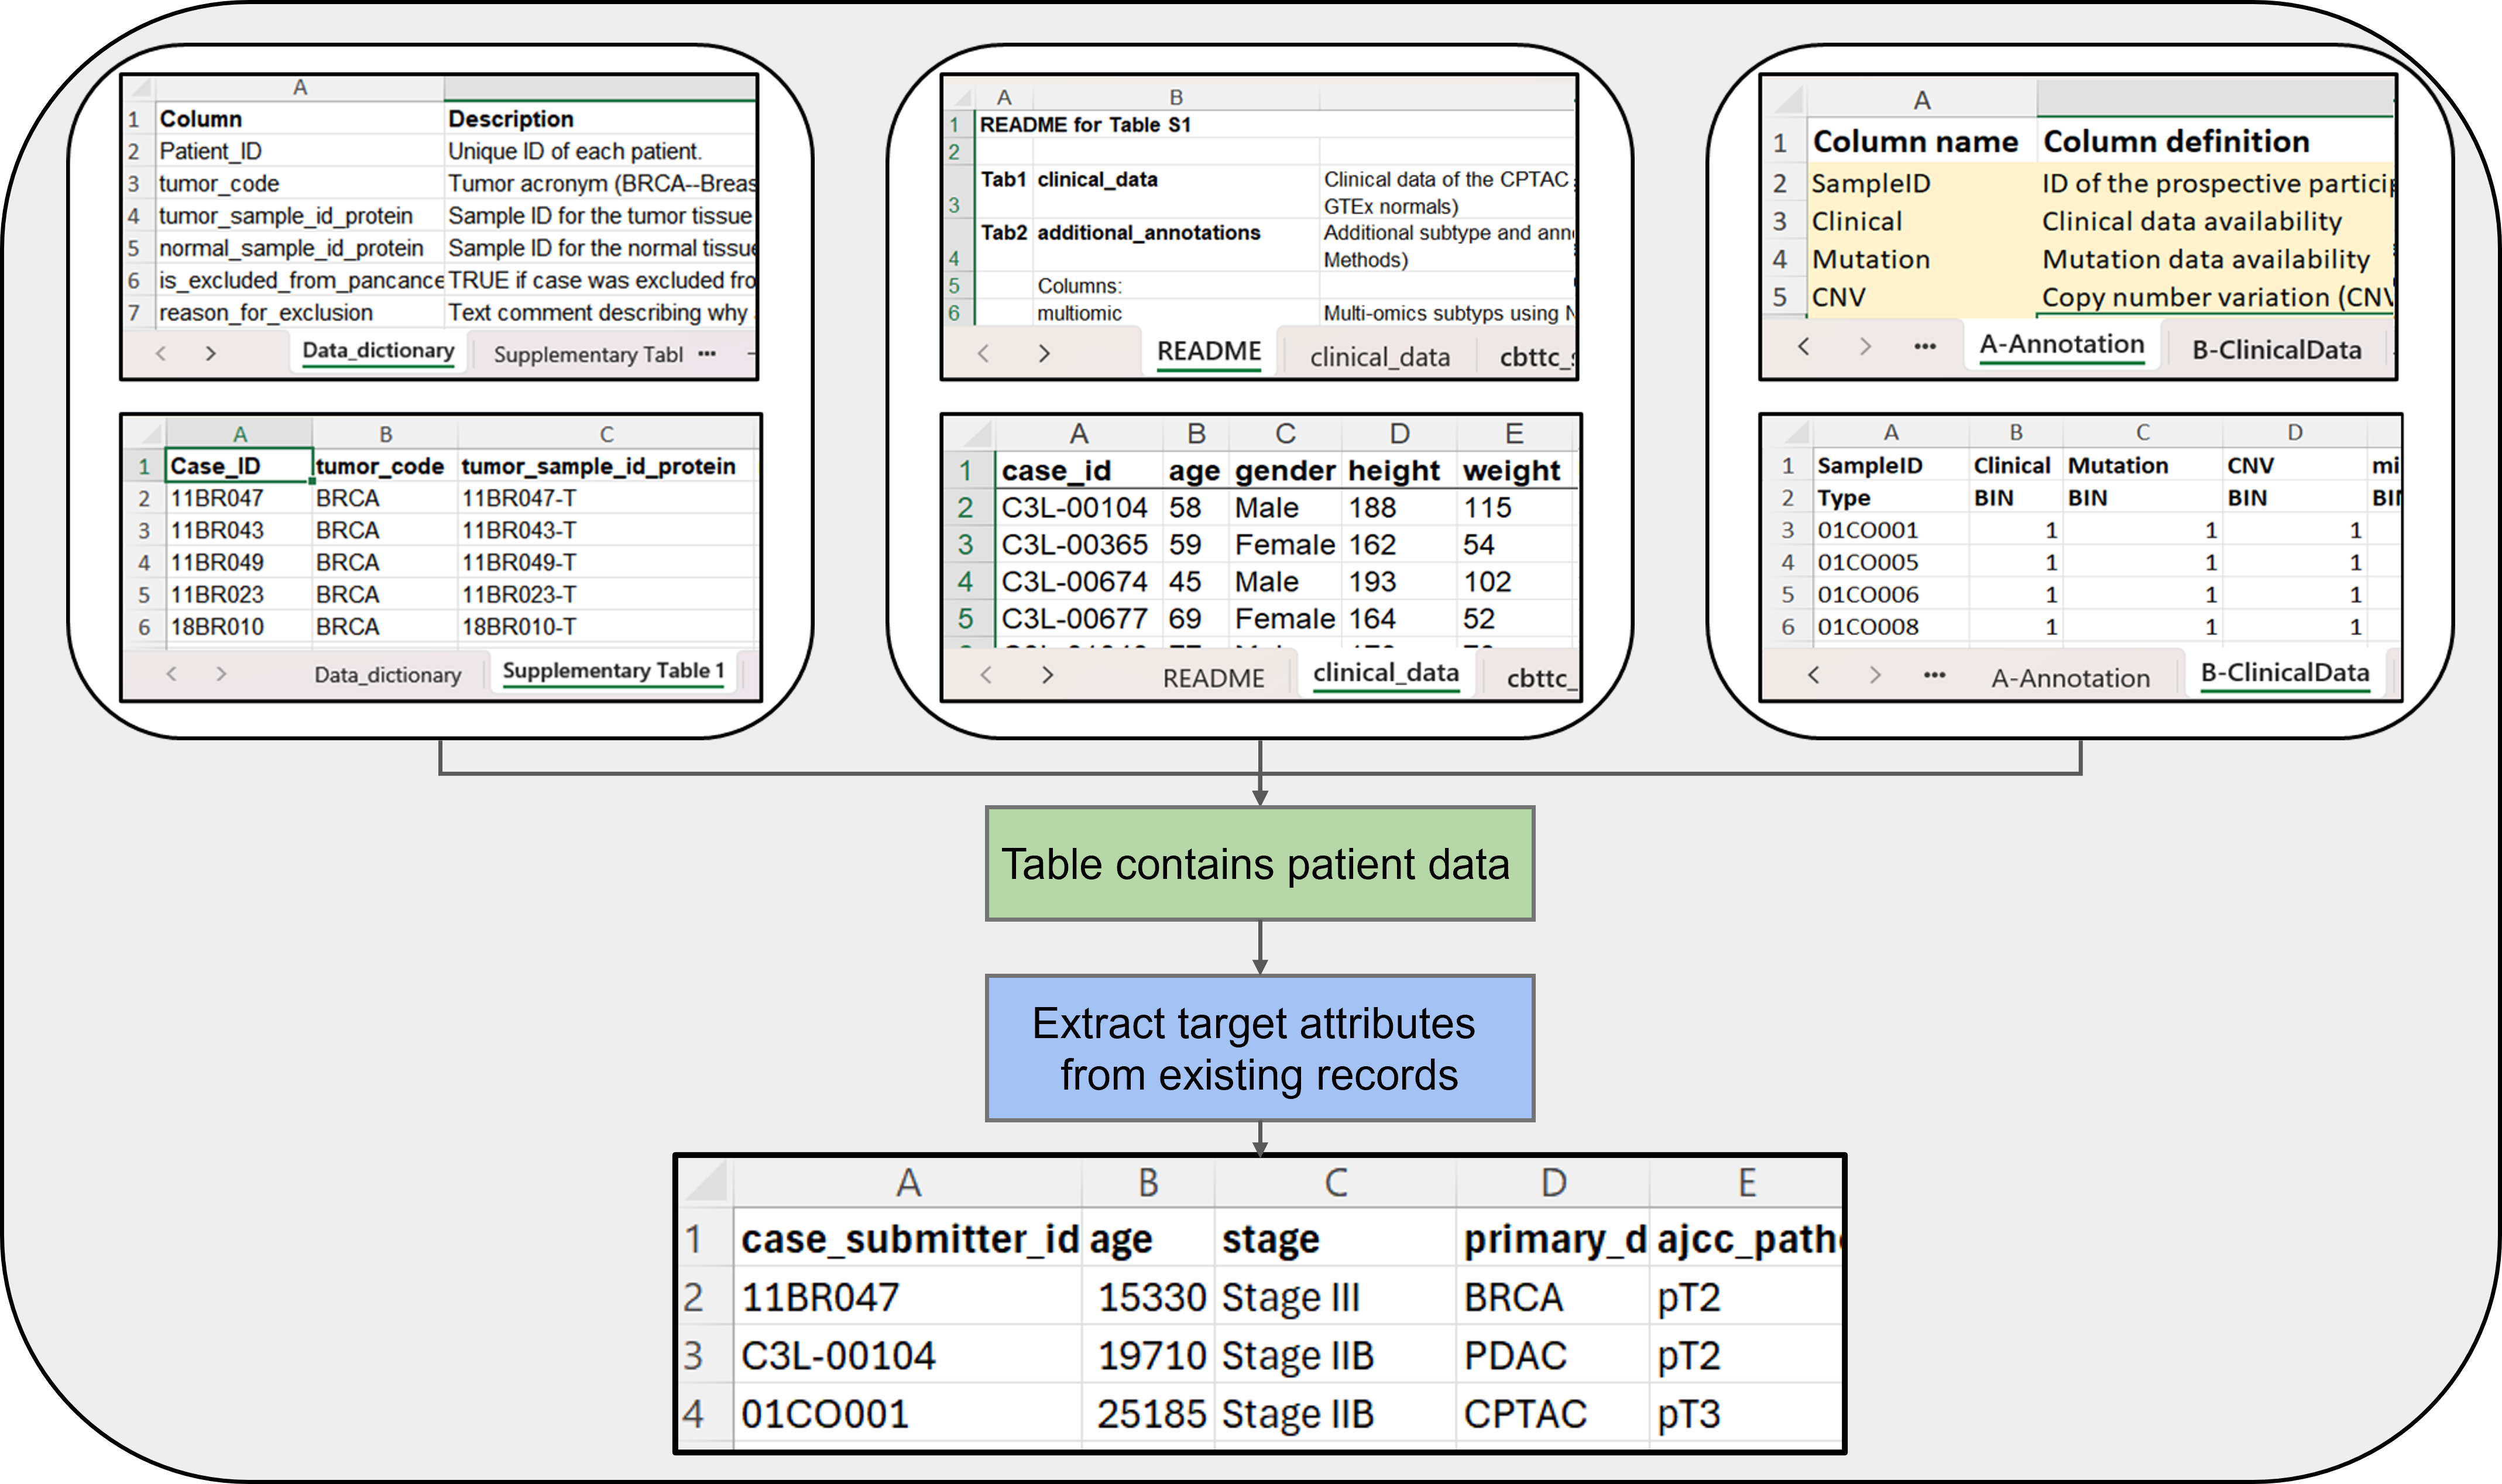
\includegraphics[width=0.8\textwidth]{imgs/biofabric_matching.png}
%     \caption{Example of the Medical Schema Matching workload. Three spreadsheets contain several tables and \system{} (1) filters for tables that relate to patient data and (2) matches and extracts the relevant attributes, consolidating a single table with a target schema.}
%     \label{fig:biofabric-matching}
%     % \caption{}
% \end{figure*}

\begin{figure}
  \centering % breaklines
  \begin{minted}[xleftmargin=17pt,linenos,escapeinside=||,fontsize={\fontsize{8.5}{7.5}\selectfont}]{python}
import palimpzest as pz

class CaseData(|\textcolor{blue}{pz.Schema}|):
    """An individual row extracted from a table containing medical study data."""
    case_submitter_id = |\textcolor{blue}{pz.StringField}|(desc="The ID of the case")
    age_at_diagnosis = |\textcolor{blue}{pz.NumericField}|(desc="The age of the patient...", required=False)
    race = |\textcolor{blue}{pz.StringField}|(desc="An arbitrary classification of a...", required=False)
    ethnicity = |\textcolor{blue}{pz.StringField}|(desc="Whether an individual...", required=False)
    gender = |\textcolor{blue}{pz.StringField}|(desc="Text designations that identify gender.", required=False)
    vital_status = |\textcolor{blue}{pz.StringField}|(desc="The vital status of the patient", required=False)
    ajcc_pathologic_t = |\textcolor{blue}{pz.StringField}|(desc="The AJCC pathologic T", required=False)
    ajcc_pathologic_n = |\textcolor{blue}{pz.StringField}|(desc="The AJCC pathologic N", required=False)
    ajcc_pathologic_stage = |\textcolor{blue}{pz.StringField}|(desc="The AJCC pathologic stage", required=False)
    tumor_grade = |\textcolor{blue}{pz.StringField}|(desc="The tumor grade", required=False)
    tumor_focality = |\textcolor{blue}{pz.StringField}|(desc="The tumor focality", required=False)
    tumor_largest_dimension_diameter = |\textcolor{blue}{pz.NumericField}|(desc="The largest...", required=False)
    primary_diagnosis = |\textcolor{blue}{pz.StringField}|(desc="The primary diagnosis", required=False)
    morphology = |\textcolor{blue}{pz.StringField}|(desc="The morphology", required=False)
    tissue_or_organ_of_origin = |\textcolor{blue}{pz.StringField}|(desc="The tissue or organ...", required=False)
    filename = |\textcolor{blue}{pz.StringField}|(desc="The name of the file...", required=False)
    study = |\textcolor{blue}{pz.StringField}|(desc="The last name of the author of the study...", required=False)


# define logical plan
xls = |\textcolor{blue}{pz.Dataset}|("medical-eval", schema=|\textcolor{blue}{pz.XLSFile}|)
patient_tables = xls.convert(
    |\textcolor{blue}{pz.Table}|, desc="All tables in the file", cardinality="oneToMany"
)
patient_tables = patient_tables.filter("The rows of the table contain the patient age")
case_data = patient_tables.convert(
    CaseData, desc="The patient data in the table", cardinality="oneToMany"
)

# create and execute physical plans...
    \end{minted}
  \caption{The AI program written using \system{} for the Medical Schema Matching workload. 
  % In the program snippet above, we show the definition of the (\system{}) schemas and the creation of the logical plan. We then created a set of physical plans, executed each one, and recorded the runtime, cost, and quality of each plan.
  }
  \label{fig:medical-schema-matching-program}
\end{figure}

